\documentclass[13pt]{book}

% list all the packages used
\usepackage[utf8]{inputenc}
\usepackage{amssymb}
\usepackage{mathtools}
\usepackage{amsmath}
\usepackage{verbatim}
\usepackage{tikz}
\usetikzlibrary{arrows.meta}

\tikzset{%
  >={Latex[width=2mm,length=2mm]},
  % Specifications for style of nodes:
            base/.style = {rectangle, rounded corners, draw=black,
                           minimum width=4cm, minimum height=1cm,
                           text centered, font=\sffamily},
  activityStarts/.style = {base, fill=blue!30},
       startstop/.style = {base, fill=red!30},
    activityRuns/.style = {base, fill=green!30},
         process/.style = {base, minimum width=2.5cm, fill=orange!15,
                           font=\ttfamily},
                       }
                       
% Table of contents
\title{Machine Learning by Andrew Ng}
\author{Rangarajan R}
\date{\today}


\begin{document}

\maketitle
\tableofcontents

\mainmatter{}
\chapter{Introduction}
\section{What is machine learning}
\begin{itemize}
\item \textbf{Machine Learning definition} \\
  \(\rightarrow\) Arthur Samuel (1959). Field of study that gives computers the ability to learn without being explicity programmed. \\
  \(\rightarrow\)Tom Mitchell(1998) Well-posed Learning Problem. A computer program is said to \emph{learn} from experience \textbf{E} with respect to some task \textbf{T} and some performance measure \textbf{P}, if its performance on \textbf{T}, as measured by \textbf{P}, improves with experience \textbf{E}.
\item Suppose your email program watches which emails you do or do not mark as spam, and based on that learns how to better filter spam. What is the task \textbf{T} in this setting \(?\)
  \begin{enumerate}
\item Classifying emails as spam or not spam. \(\rightarrow\) \textbf{T}
\item Watching you label emails as spam or not spam. \(\rightarrow\) \textbf{E}
\item The number(or fraction) of emails correctly classified as spam/not spam. \(\rightarrow\) \textbf{P}
\item None of the above this is not a machine learning problem.
  \end{enumerate}
\item \textbf{Machine learning algorithms}
  \begin{enumerate}
\item Supervised learning
\item Unsupervised learning
\item Other \(:\)Reinforcement learning and recommender systems
  \end{enumerate}
\end{itemize}
\section{Supervised Learning}
\begin{itemize}
  \item Supervised learning \(:\) right answers given.
  \item \textbf{Regression:} Predict continuous valued output.
  \item \textbf{Classification:} Discrete valued output.
  \item You\'re running a company, and you want to develop learning algorithms to address each of two problems.
  \item Problem 1 You have a large inventory system of identical items. You want to predict how many of these items will sell over the next 3 months. \(\rightarrow\) \textbf{regression problem}
  \item Problem 2 You\'d like software to examine individual customer accounts, and for each account decide if it has been hacked/cimpromised. \(\rightarrow\) \textbf{classification problem}
\end{itemize}

\section{Unsupervised Learning}
\begin{itemize}
\item Application \(:\)
  \begin{enumerate}
    \item Organize computer clusters
    \item Social networking analysis
    \item Market segmentation
    \item Astronomical data analysis
  \end{enumerate}
\item Of the following examples, which would you address using an unsupervised learning algorithm \(?\) Check all that apply.
  \begin{enumerate}
    \item Given email labelled as spam/not spam, learn a spam filter. \(\rightarrow\) \textbf{Supervised learning}
    \item Given a set of news articles found on the web, group them into a set of articles about the same story. \(\rightarrow\) \textbf{Unsupervised learning}
    \item Given a database of customer data, automatically discover market segments and group customers into different market segments. \(\rightarrow\) \textbf{Unsupervised learning}
    \item Given a dataset of patients diagonised as either having diabetes or not, learn to classify new patients having diabetes or not. \(\rightarrow\) \textbf{Supervised learning}
  \end{enumerate}
  
\end{itemize}

\chapter{Linear Regression with one variable}

\section{Model representation}
\begin{itemize}
\item Notations \(:\)
  \begin{itemize}
  \item [\textbf{m = }] Number of training examples
  \item [\textbf{x's = }] input variable/features
  \item[\textbf{y's = }] output variable/target variable
  \item [\textbf{(x,y) = }] one training example
  \item [\textbf{(x}\(^{ith}\)\textbf{,y}\(^{ith}\)) = ] i\(^{th}\) training example
    \end{itemize}
  \item Model representation
% Drawing part, node distance is 1.5 cm and every node
% is prefilled with white background
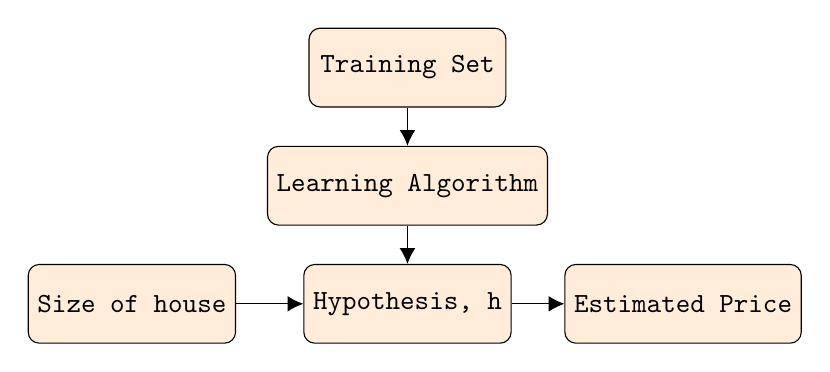
\begin{tikzpicture}[node distance=1.5cm,
    every node/.style={fill=white, font=\sffamily}, align=center]
  % Specification of nodes (position, etc.)
  \node (start)             [process]              {Training Set};
  \node (LearningAlgorithm) [process, below of=start]          {Learning Algorithm};
  \node (Hypothesis)      [process, below of=LearningAlgorithm]   {Hypothesis, h};
  \node (SizeHouse)     [process, left of=Hypothesis, xshift=-2cm]   {Size of house};
  \node (EstimatedPrice)     [process, right of=Hypothesis, xshift=2cm]   {Estimated Price};
  
  % Specification of lines between nodes specified above
  % with aditional nodes for description 
  \draw[->]             (start) -- (LearningAlgorithm);
  \draw[->]     (LearningAlgorithm) -- (Hypothesis);
  \draw[->]      (SizeHouse) -- (Hypothesis);
  \draw[->]      (Hypothesis) -- (EstimatedPrice);  
\end{tikzpicture}
\item How do we represent h
  \begin{equation}
    h_\theta = \theta_0 + \theta_1x
  \end{equation}
  
\item Linear regression with one variable. Univariate linear regression.
\end{itemize}

\section{Cost function}
\begin{itemize}
\item Hypothesis{:}
    \begin{equation}
    h_\theta(x) = \theta_0 + \theta_1x
  \end{equation}
\item Parameters{:}
  \(\theta_0, \theta_1\)
\item Cost Function{:}
  \begin{equation}
    h(\theta_0,\theta_1) = \frac{1}{2m}\sum_{i=1}^m(h_\theta(x^{(i)}) - y^{(i)})^2
  \end{equation}
  \item Goal{:} minimize\(J(\theta_0, \theta_1)\)
\item Idea {:}
  Choose \(\theta_0, \theta_1\) so that \(h_0(x)\) is so close to y for our training examples(x,y)
\end{itemize}

\section{Gradient descent}
\begin{itemize}
  \item Have some function \(J(\theta_0, \theta_1)\) 
  \item Want minimize \(J(\theta_0, \theta_1)\) 
  \item Start with some \(\theta_0, \theta_1\)
  \item Keep changing \(\theta_0, \theta_1\) to reduce \(J(\theta_0, \theta_1)\) until we hopefully end up at a minimum.
\end{itemize}
 \subsection{Gradient descent algorithm}
 \begin{itemize}
 \item repeat until convergence \{
   \begin{equation}
     \theta_j := \theta_j - \alpha\frac{\partial}{\partial\theta_j}J(\theta_0, \theta_1)
   \end{equation}
    (for j = 0 and j = 1)
 \}
\item Correct{:} Simultaneous update
   \begin{equation}
     temp0 := \theta_0 - \alpha\frac{\partial}{\partial\theta_0}J(\theta_0, \theta_1)
   \end{equation}
   \begin{equation}
     temp1 := \theta_1 - \alpha\frac{\partial}{\partial\theta_1}J(\theta_0, \theta_1)
   \end{equation}
   \begin{equation}
     \theta_0 := temp0
   \end{equation}
   \begin{equation}
     \theta_1 := temp1 
   \end{equation}
  where \(\alpha\) is the learning rate
\item Consider
   \begin{equation}
     temp1 := \theta_1 - \alpha\frac{\partial}{\partial\theta_1}J(\theta_0, \theta_1)
   \end{equation}
   \begin{enumerate}
   \item If \(\alpha\) is too small, gradient descent can be slow.
   \item If \(\alpha\) is too large, gradient descent can overshoot the minimum. It may fail to converge, or even diverge.
   \item Gradient descent can converge to a local minimum, even with the learning rate \(\alpha\) fixed.
   \item As we approach a local minimum, gradient descent will automatically take smaller steps. So, no need to decrease \(\alpha\) over time.
     \end{enumerate}
 \item repeat until convergence \{
   \begin{equation}
     \theta_0 := \theta_0 - \alpha\frac{1}{m}\sum_{i=1}^m(h_\theta(x^{(i)}) - y^{(i)})
   \end{equation}
   \begin{equation}
     \theta_1 := \theta_1 - \alpha\frac{1}{m}\sum_{i=1}^m(h_\theta(x^{(i)}) - y^{(i)}).x^{(i)}     
   \end{equation}
    \}
 \item Batch Gradient Descent {:}
   Each step of gradient descent uses all the training examples.
  
  \end{itemize}

\chapter{Linear Regression with multiple variables}
\begin{itemize}
  \item
\end{itemize}

\section{Multiple features}
\begin{itemize}
  \item
\end{itemize}

\section{Gradient descent for multiple variables}
\begin{itemize}
  \item
\end{itemize}

\section{Feature scaling}
\begin{itemize}
  \item
\end{itemize}

\section{Learning rate}
\begin{itemize}
  \item
\end{itemize}

\section{Features and polynomial regression}
\begin{itemize}
  \item
\end{itemize}

\section{Normal equation}
\begin{itemize}
  \item
\end{itemize}

\chapter{Logistic Regression}
\begin{itemize}
  \item
\end{itemize}

\section{Classification}
\begin{itemize}
  \item
\end{itemize}

\section{Hypothesis Representation}
\begin{itemize}
  \item
\end{itemize}

\section{Decision boundary}
\begin{itemize}
  \item
\end{itemize}

\section{Cost function}
\begin{itemize}
  \item
\end{itemize}

\section{Advanced optimisation}
\begin{itemize}
  \item
\end{itemize}

\section{Multiclass classification}
\begin{itemize}
  \item
\end{itemize}

\section{The problem of overfitting}
\begin{itemize}
  \item
\end{itemize}

\chapter{Regularization}
\begin{itemize}
  \item
\end{itemize}

\section{Cost function}
\begin{itemize}
  \item
\end{itemize}

\section{Regularized linear regression}
\begin{itemize}
  \item
\end{itemize}

\section{Regularized logistic regression}
\begin{itemize}
  \item
\end{itemize}

\chapter{Neural Networks}
\begin{itemize}
  \item
\end{itemize}

\section{Non-linear hypotheses}
\begin{itemize}
  \item
\end{itemize}

\section{Neurons and the brain}
\begin{itemize}
  \item
\end{itemize}

\section{Model representation}
\begin{itemize}
  \item
\end{itemize}

\section{Multi-class classification}
\begin{itemize}
  \item
\end{itemize}

\section{Cost function}
\begin{itemize}
  \item
\end{itemize}

\section{Back propagation algorithm}
\begin{itemize}
  \item
\end{itemize}

\section{Implementation note Unrolling parameters}
\begin{itemize}
  \item
\end{itemize}

\section{Gradient checking}
\begin{itemize}
  \item
\end{itemize}

\section{Random initialization}
\begin{itemize}
  \item
\end{itemize}

\chapter{Advice for applying machine learning}
\begin{itemize}
  \item
\end{itemize}

\section{Deciding what to try next}
\begin{itemize}
  \item
\end{itemize}

\section{Evaluating a hypothesis}
\begin{itemize}
  \item
\end{itemize}

\section{Model selection and training, validation, test sets}
\begin{itemize}
  \item
\end{itemize}

\section{Diagnosing bias vs variance}
\begin{itemize}
  \item
\end{itemize}

\section{Regularization and bias,variance}
\begin{itemize}
  \item
\end{itemize}

\section{Learning curves}
\begin{itemize}
  \item
\end{itemize}

\chapter{Machine learning system design}
\begin{itemize}
  \item
\end{itemize}

\section{Error analysis}
\begin{itemize}
  \item
\end{itemize}

\section{Error metrics for skewed classes}
\begin{itemize}
  \item
\end{itemize}

\section{Trading off precision and recall}
\begin{itemize}
  \item
\end{itemize}

\section{Data for machine learning}
\begin{itemize}
  \item
\end{itemize}

\chapter{Support Vector Machines}
\begin{itemize}
  \item
\end{itemize}

\section{Optimisation objective}
\begin{itemize}
  \item
\end{itemize}

\section{Large margin}
\begin{itemize}
  \item
\end{itemize}

\section{Kernels}
\begin{itemize}
  \item
\end{itemize}

\section{Using an SVM}
\begin{itemize}
  \item
\end{itemize}

\chapter{Clustering}
\begin{itemize}
  \item
\end{itemize}

\section{Unsupervised learning introduction}
\begin{itemize}
  \item
\end{itemize}

\section{K-means algorithm}
\begin{itemize}
  \item
\end{itemize}

\section{Optimisation objective}
\begin{itemize}
  \item
\end{itemize}

\section{Random initialization}
\begin{itemize}
  \item
\end{itemize}

\section{Choosing the number of clusters}
\begin{itemize}
  \item
\end{itemize}

\chapter{Dimensionality Reduction}
\begin{itemize}
  \item
\end{itemize}

\section{Data Compression}
\begin{itemize}
  \item
\end{itemize}

\section{Data Visualization}
\begin{itemize}
  \item
\end{itemize}

\section{Principal Component Analysis problem formulation}
\begin{itemize}
  \item
\end{itemize}

\section{Principal Component Analysis algorithm}
\begin{itemize}
  \item
\end{itemize}

\section{Choosing the number of principal components}
\begin{itemize}
  \item
\end{itemize}

\section{Reconstructed from compressed representation}
\begin{itemize}
  \item
\end{itemize}

\chapter{Anomaly detection}
\begin{itemize}
  \item
\end{itemize}

\section{Problem motivation}
\begin{itemize}
  \item
\end{itemize}

\section{Guassian distribution}
\begin{itemize}
  \item
\end{itemize}

\section{Algorithm}
\begin{itemize}
  \item
\end{itemize}

\section{Anomaly detection vs supervised learning}
\begin{itemize}
  \item
\end{itemize}

\section{Choosing what features to use}
\begin{itemize}
  \item
\end{itemize}

\section{Multivariate Guassian distribution}
\begin{itemize}
  \item
\end{itemize}

\section{Developing and evaluating an anomaly detection system}
\begin{itemize}
  \item
\end{itemize}

\chapter{Large scale machine learning}
\begin{itemize}
  \item
\end{itemize}

\section{Learning with large datasets}
\begin{itemize}
  \item
\end{itemize}

\section{Stochastic gradient descent}
\begin{itemize}
  \item
\end{itemize}

\section{Mini-batch gradient descent}
\begin{itemize}
  \item
\end{itemize}

\section{Stochastic gradient descent convergence}
\begin{itemize}
  \item
\end{itemize}

\section{Map-reduce and data parallelism}
\begin{itemize}
  \item
\end{itemize}

\chapter{Application examples}
\begin{itemize}
  \item
\end{itemize}

\section{Problem description and pipeline}
\begin{itemize}
  \item
\end{itemize}

\section{Sliding windows}
\begin{itemize}
  \item
\end{itemize}

\section{Getting lots of data Artifical data synthesis}
\begin{itemize}
  \item
\end{itemize}

\section{Ceiling analysis What part of the pipeline to work on next}
\begin{itemize}
  \item
\end{itemize}

\end{document}
